\chapter{Случайные величины}

\section{Сформулировать определение случайной величины и функции распределения вероятностей случайной величины. Доказать свойства функции распределения.}

Пусть $(\Omega, \beta, P)$ -- вероятностное пространство некоторого случайного эксперимента.

\textbf{Случайной величиной} называется функция $X: \Omega \rightarrow \mathbb{R}$ такая, что $\forall x \in \mathbb{R}: \{\omega: X(\omega) < x\} \in \beta$.

\textbf{Функцией распределения вероятностей случайной величины} $X$ называется отображение $F_X:~\mathbb{R}\rightarrow\mathbb{R}$, определенное правилом $F_X(x) = P\{X < x\}$.

\subsection*{Свойства функции распределения}
\begin{enumerate}
	\item $0 \leq F(x) \leq 1$.
	
		\textbf{Доказательство.} $F(x)$ определена как вероятность, т.е. $F(x) = P\{...\} \in [0; 1]$.
		
	\item $F$ -- неубывающая функция, т.e. если $x_1 \leq x_2$, то $F(x_1) \leq F(x_2).$
	
		\textbf{Доказательство.} Если $x_1 \leq x_2$, тогда $F(x_2) = P\{X < x_2\} = P\{\underbrace{\{X < x_1\}}_\text{Событие $A$} + \underbrace{\{x_1 \leq X < x_2\}}_\text{Событие $B$}\}$. События $A$ и $B$ несовместны $\Rightarrow F(x_2) = P\{\underbrace{\{X < x_1\}}_\text{$F(x_1)$} + \underbrace{\{x_1 \leq X < x_2\}}_\text{$\geq0$}\} \geq F(x_1)$.  
	
	\item  $\lim\limits_{x \rightarrow -\infty}F(x) = 0$; $\lim\limits_{x \rightarrow +\infty}F(x) = 1$.
	
		\textbf{Доказательство.} Рассмотрим последовательность $x_1, x_2, x_3,...$ такую, что 
		
		(a) $x_1 < x_2 < x_3 < ...$; 
		
		(b) $\lim\limits_{i \rightarrow \infty} x_i = +\infty$.
		
		$A_i = \{X < x_i\}, i \in \mathbb{N}$; $A_1 \subseteq A_2 \subseteq ... \subseteq A_n \subseteq A_{n+1} \subseteq ...$ -- неубывающая последовательность событий. $\Rightarrow \lim\limits_{x \rightarrow \infty} F(x_i) = \lim\limits_{i \rightarrow \infty} P(A_i) = |\text{аксиома непрерывности}| = P\{X < +\infty\} = 1$.
		
		Т.к. $x_1, x_2, x_3,...$ -- произвольная последовательность (неубывающая и стремящаяся к бесконечности), то в соответствии с определением предела функции по Гейне $\lim\limits_{x \rightarrow +\infty}F(x) = 1$. Вторая часть этого свойства доказывается аналогично.
		
	\item $\lim\limits_{x \rightarrow x_0-}F(x) = F(x_0)$, в каждой точке $F$ непрерывна слева.
		
		\textbf{Доказательство.} Пусть $x_1,x_2,...$ -- возрастающая последовательность, $\lim\limits_{i \rightarrow \infty}x_i = x_0$.
		
		Пусть $A_i = \{X < x_i\}, i \in \mathbb{N}$. Тогда событие $\{X < x_i\} = \bigcup_{i=1}^\infty A_i$, причем последовательность событий $A_1,A_2,...$ является возраставющей $\Rightarrow \lim\limits_{i \rightarrow \infty} F(x_i) = \lim\limits_{i \rightarrow \infty} P(A_i) = |\text{аксиома непрерывности}|=P\{X<x_0\} = F(x_0)$. Т.к. $x_1, x_2,...$ - произвольная последовательность, сходящаяся к $x_0$ слева, то в соответствии с определением предела функции по Гейне $\lim\limits_{x \rightarrow x_0-} F(x) = F(x_0)$.
		
	\item $P\{a \leq X < b\} = F(b) - F(a)$.
	
		\textbf{Доказательство.} $\{X < b\} = \{X < a\} + \{a \leq X < b\} \Rightarrow \underbrace{P\{X < b\}}_\text{$F(b)$} = \underbrace{P\{X < a\}}_\text{$F(a)$} +$\newline $+P\{a \leq X < b\} \Rightarrow P\{a~\leq~X~<~b\}~=~F(b) - F(a)$.
\end{enumerate}

\section{Сформулировать определения случайной величины и функции распределения случайной величины. Сформулировать определения дискретной и непрерывной случайной величины. Доказать свойства плотности распределения вероятностей непрерывной случайной величины.}

Пусть $(\Omega, \beta, P)$ -- вероятностное пространство некоторого случайного эксперимента.

\textbf{Случайной величиной} называется функция $X: \Omega \rightarrow \mathbb{R}$ такая, что $\forall x \in \mathbb{R}: \{\omega: X(\omega) < x\} \in \beta$.

\textbf{Функцией распределения вероятностей случайной величины} $X$ называется отображение $F_X:~\mathbb{R}\rightarrow\mathbb{R}$, определенное правилом $F_X(x) = P\{X < x\}$.

Случайная величина называется \textbf{дискретной}, если множество её значений конечно или счётно.

Случайная величина $X$ называется \textbf{непрерывной}, если существует функция $f(x): \mathbb{R} \rightarrow \mathbb{R}$ такая, что $\forall x \in \mathbb{R}: F(x) = \int_{-\infty}^{x}f(t)dt$ ($F$ -- функция распределения вероятностей случайной величины $X$). При этом $f$ называют функцией плотности распределения вероятности случайной величины $X$.

\subsection*{Cвойства плотности распределения вероятностей}
\begin{enumerate}
	\item $f(x) \geq 0$.
	
		\textbf{Доказательство.} $F$ -- неубывающая функция $\Rightarrow f(x) = F^\text{'}(x) \geq 0$.
	
	\item $P\{a \leq X < b\} = \int_{a}^{b}f(x)dx$.
	
		\textbf{Доказательство.} $P\{x \leq X < b\} = F(b) - F(a) = [f(x)=F^\text{'}(x); \text{по формуле Ньютона--Лейбница}] = \text{$=$}\int_{a}^{b}f(x)dx$. 
	
	\item $\int_{-\infty}^{+\infty}f(x)dx = 1$.
	
		\textbf{Доказательство.} $\int_{-\infty}^{+\infty}f(x)dx = \lim\limits_{\substack{x_1 \rightarrow -\infty \\ x_2 \rightarrow +\infty}} \int_{x_1}^{x_2}f(x)dx = |\text{свойство 2}| = \lim\limits_{x_2 \rightarrow +\infty}F(x_2) - \lim\limits_{x_1 \rightarrow -\infty}F(x_1) =$ $=F(+\infty)-F(-\infty)=1-0=1$.
	
	\item $P\{x_0 \leq X < x_0 + \Delta x\} \approx f(x_0)\Delta x$; $x_0$ -- точка непрерывности функции $f$, $\Delta x$ -- мало.
	
		\textbf{Доказательство.} $P\{x_0 \leq X < x_0 + \Delta x\} = |\text{свойство 2}| = F(x_0 + \Delta x) - F(x_0)$. Т.к. $x_0$ -- точка непрерывности $f$, а $\Delta x$ -- мало, то можно считать, что в окрестности $(x_0, x_0 + \Delta x)$ функция $F^\text{'} = f$ непрерывна. Применим к функции $f$ на $[x_0, x_0 + \Delta x]$ т. Лагранджа $F(x_0 + \Delta x) - F(x_0) = \underbrace{F^\text{'}(\xi)}_\text{$f(\xi)$}\Delta x$, где $\xi \in (x_0, x_0 + \Delta x)$. Т.к. $\Delta x$ мало, а $f$ непрерывна в некоторой окрестности $x_0$, то можно считать, что $f(\xi) \approx f(x_0)$. Таким образом, $P\{x_0 \leq X < x_0 + \Delta x\} \approx f(x_0)\Delta x$.
	
	\item Для любого наперед заданного $x_0 \in \mathbb{R}$: $P\{X = x_0\} = 0$.
	
		\textbf{Доказательство.} $P\{X=x_0\}=\lim\limits_{\Delta x \rightarrow 0} P\{x_0 \leq X < x_0 + \Delta x\} = \lim\limits_{\Delta x \rightarrow 0}[F(x_0 + \Delta x) - F(x_0)] = 0$, т.к. $F$ -- непрерывна.
		
\end{enumerate}

\section{Сформулировать определение нормальной случайной величины, указать геометрический смысл параметров. Понятие стандартного нормального закона. Доказать формулу для вычисления вероятности попадания нормальной случайной величины в интервал.}

Говорят, что случайная величина $X$ имеет \textbf{нормальное распределение} с параметрами $m$ и $\sigma^2 (\sigma > 0)$, если её функция плотности имеет вид $f(x) = \frac{e^{-\frac{(x-m)^2}{2\sigma^2}}}{\sigma\sqrt{2\pi}}, x \in \mathbb{R}$. Обозначается $X ~ N(m, \sigma^2)$.


\begin{figure}[ht!]
	\begin{minipage}{0.4\textwidth}
		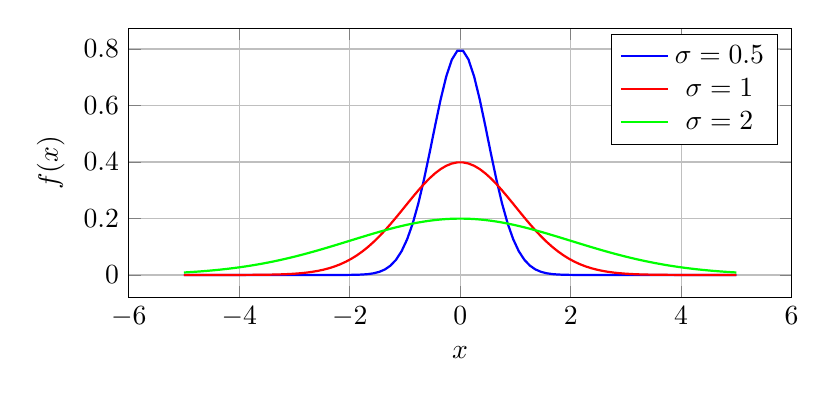
\begin{tikzpicture}
			\begin{axis}[domain=-5:5, width=10cm, height=5cm, grid, xlabel={$x$}, ylabel={$f(x)$}]
				\addplot[blue, thick, samples=100] {exp(-((x-0)^2)/(2*(0.5)^2))/(0.5*sqrt(2*pi))};
				\addplot[red, thick, samples=100] {exp(-((x-0)^2)/(2*(1)^2))/(1*sqrt(2*pi))};
				\addplot[green, thick, samples=100] {exp(-((x-0)^2)/(2*(2)^2))/(2*sqrt(2*pi))};
				\legend{$\sigma = 0.5$, $\sigma = 1$, $\sigma = 2$}
			\end{axis}
		\end{tikzpicture}
	\end{minipage}%
	\hfill
	\begin{minipage}{0.45\textwidth}
		Функция плотности нормального распределения имеет характерную колоколообразную форму; $m$ является координатой $x$ <<центра>> этого колокола (центра симметрии), а $\sigma$ характеризует разброс значений случайной величины; чем меньше $\sigma$, тем выше экстремум функции плотности.
	\end{minipage}
\end{figure}

Распределение $N(0, 1)$ называет \textbf{стандартным нормальным распределением}; для него функция плотности равна $f(x) = \frac{e^{-\frac{x^2}{2}}}{\sqrt{2\pi}}, x \in \mathbb{R}$.

\subsection*{Формула для вычисления вероятности попадания нормальной случайной величины в интервал.}

Рассмотрим
\[
P\{a \leq X < b\} = \Bigl\langle \text{по свойству плотности распределения} \Bigr\rangle =
\int_a^b f_X(x) \, dx = \int_a^b \frac{1}{\sigma \sqrt{2\pi}} e^{-\frac{(x - m)^2}{2\sigma^2}} \, dx =
\]
\[
= \Bigl\langle t = \frac{x - m}{\sigma}, \, dx = \sigma \, dt; \, x = a \implies t = \frac{a - m}{\sigma}, \, x = b \implies t = \frac{b - m}{\sigma} \Bigr\rangle =
\]
\[
= \int_{\frac{a-m}{\sigma}}^{\frac{b-m}{\sigma}} \frac{1}{\sqrt{2\pi}} e^{-\frac{t^2}{2}} \, dt = \Bigl\langle \Phi(t) = \int_{-\infty}^t f_{0,1}(t) \, dt \Bigr\rangle =
\]
\[
= \Phi\left(\frac{b - m}{\sigma}\right) - \Phi\left(\frac{a - m}{\sigma}\right) = \Bigl\langle \Phi(t) \text{ — стандартное нормальное распределение, такое, что }
\]
\[
\Phi(0) = \frac{1}{2} \implies \Phi(t) \Bigr\rangle = \Phi_0\left(\frac{b - m}{\sigma}\right) - \Phi_0\left(\frac{a - m}{\sigma}\right).
\]

Т.к. \( X \sim N(m, \sigma^2) \) — непрерывная случайная величина, то
\[
P\{a \leq X \leq b\} = \Phi_0\left(\frac{b - m}{\sigma}\right) - \Phi_0\left(\frac{a - m}{\sigma}\right) = \Phi\left(\frac{b - m}{\sigma}\right) - \Phi\left(\frac{a - m}{\sigma}\right).
\]

\section{Сформулировать определение случайного вектора и функции распределения вероятностей случайного вектора. Сформулировать свойства функции распределения двумерного случайного вектора. Доказать предельные свойства.}

Пусть: 
\begin{enumerate}
	\item $(\Omega, \beta, P)$ -- вероятностное пространство.
	
	\item $X_{\omega} = X_1(\omega),...,X_n(\omega)$ -- случайные величины, заданные на этом вероятностном пространстве.
\end{enumerate}
Тогда $n$-мерным \textbf{случайным вектором} называется кортеж $\vec{X} = (X_1,..., X_n)$.

\textbf{Функцией распределения вероятностей случайного вектора} называют отображение $F: \mathbb{R}^n \rightarrow \mathbb{R}$, определенное правилом $F(x_1, ..., x_n) = P\{X_1 < x_1,..., X_n < x_n\}$.

\subsection*{Свойства}
\begin{enumerate}
	\item $0 \leq F(x_1, x_2) \leq 1$.
	
	\item (a) При фиксированном $x_2$ функция $F(x_1, x_2)$ как функция переменного $x_1$
	является неубывающей функцией;
	
	(b) При фиксированном $x_1$ функция $F(x_1, x_2)$ как функция переменного $x_2$
	является неубывающей функцией;
	
	\item $\quad \lim\limits_{\substack{x_1 \to -\infty \\ x_2 = \text{const}}} F(x_1, x_2) = 0, \quad \lim\limits_{\substack{x_1 = \text{const} \\ x_2 \to -\infty}} F(x_1, x_2) = 0$.
	
		\textbf{Доказательство.} По определению, \( F(x_1, x_2) = P(\{X_1 < x_1\} \cdot \{X_2 < x_2\}) \); при \( x_1 \to -\infty \) событие \(\{X_1 < -\infty\}\) является невозможным. Произведение невозможного события на событие \(\{X_2 < x_2\}\) является невозможным событием, поэтому \( F(x_1, x_2) \) стремится к нулю при \( x_1 \to -\infty, \, x_2 = \text{const} \).
		
		$
		\lim\limits_{\substack{x_1 = \text{const} \\ x_2 \to -\infty}} F(x_1, x_2) = 0
		$ доказывается аналогично.
	
	\item $\quad \lim\limits_{\substack{x_1 \to +\infty \\ x_2 \to +\infty}} F(x_1, x_2) = 1.$.
	
		\textbf{Доказательство.} По определению, \( F(x_1, x_2) = P(\{X_1 < x_1\} \cdot \{X_2 < x_2\}) \). Событие $\{X_1 < +\infty\}$ является достоверным, $\{X_2 < +\infty\}$ также является достоверным, а произведение достоверных событий -- достоверное событие.
		
	\item $\quad \lim\limits_{{\substack{x_1 \to +\infty \\ x_2 = \text{const}}}} F(x_1, x_2) = F_{X_2}(x_2), \quad \lim\limits_{\substack{x_1 = \text{const} \\ x_2 \to +\infty}} F(x_1, x_2) = F_{X_1}(x_1)$, 
	
	где $F_{X_i}$ -- маргинальная функция распределения случайной величины $X_i$.
	
		\textbf{Доказательство.} По определению, \( F(x_1, x_2) = P(\{X_1 < x_1\} \cdot \{X_2 < x_2\})\). Событие $\{X_2 < +\infty\}$ является достоверным, следовательно, $\quad \lim\limits_{{\substack{x_1 \to +\infty \\ x_2 = \text{const}}}} F(x_1, x_2) = P\{X_2 < x_2\} = F_{X_2}(x_2)$. 
		
		Для второго предела -- доказывается аналогично.
		
	\item $D = \{(x, y): x \in [a_1, b_1), y \in [a_2, b_2)\}: P{a_1 \leq X < b_1, a_2 \leq Y < b_2} = F(b_1, b_2) - F(a_1, b_2) -$ $-F(a_2, b_1) + F(a_1, a_2)$.
	
	\item (a) При фиксированном $x_2$ функция $F(x_1, x_2)$ как функция переменного $x_1$
	является непрерывной слева в каждой точке;
	
	(b) При фиксированном $x_1$ функция $F(x_1, x_2)$ как функция переменного $x_2$
	является непрерывной слева в каждой точке;
	
\end{enumerate}


\section{Сформулировать определение случайного вектора и функции распределения вероятностей случайного вектора. Сформулировать свойства функции распределения двумерного случайного вектора. Доказать формулу для вычисления $P\{a_1 \leq X_1 < b1, a_2 \leq X_2 < b_2\}$.}

Пусть: 
\begin{enumerate}
	\item $(\Omega, \beta, P)$ -- вероятностное пространство.
	
	\item $X_{\omega} = X_1(\omega),...,X_n(\omega)$ -- случайные величины, заданные на этом вероятностном пространстве.
\end{enumerate}
Тогда $n$-мерным \textbf{случайным вектором} называется кортеж $\vec{X} = (X_1,..., X_n)$.

\textbf{Функцией распределения вероятностей случайного вектора} называют отображение $F: \mathbb{R}^n \rightarrow \mathbb{R}$, определенное правилом $F(x_1, ..., x_n) = P\{X_1 < x_1,..., X_n < x_n\}$.

\subsection*{Свойства}
\begin{enumerate}
	\item $0 \leq F(x_1, x_2) \leq 1$.
	
	\item (a) При фиксированном $x_2$ функция $F(x_1, x_2)$ как функция переменного $x_1$
	является неубывающей функцией;
	
	(b) При фиксированном $x_1$ функция $F(x_1, x_2)$ как функция переменного $x_2$
	является неубывающей функцией;
	
	\item $\quad \lim\limits_{\substack{x_1 \to -\infty \\ x_2 = \text{const}}} F(x_1, x_2) = 0, \quad \lim\limits_{\substack{x_1 = \text{const} \\ x_2 \to -\infty}} F(x_1, x_2) = 0$.
	
	\item $\quad \lim\limits_{\substack{x_1 \to +\infty \\ x_2 \to +\infty}} F(x_1, x_2) = 1.$.
	
	\item $\quad \lim\limits_{{\substack{x_1 \to +\infty \\ x_2 = \text{const}}}} F(x_1, x_2) = F_{X_2}(x_2), \quad \lim\limits_{\substack{x_1 = \text{const} \\ x_2 \to +\infty}} F(x_1, x_2) = F_{X_1}(x_1)$, 
	
	где $F_{X_i}$ -- маргинальная функция распределения случайной величины $X_i$.
	
	\item $D = \{(x, y): x \in [a_1, b_1), y \in [a_2, b_2)\}: P\{a_1 \leq X < b_1, a_2 \leq Y < b_2\} = F(b_1, b_2) - F(a_1, b_2) -$ $-F(a_2, b_1) + F(a_1, a_2)$.
	
	\item (a) При фиксированном $x_2$ функция $F(x_1, x_2)$ как функция переменного $x_1$
	является непрерывной слева в каждой точке;
	
	(b) При фиксированном $x_1$ функция $F(x_1, x_2)$ как функция переменного $x_2$
	является непрерывной слева в каждой точке;
	
\end{enumerate}

\subsection*{Формула для вычисления $P\{a_1 \leq X_1 < b1, a_2 \leq X_2 < b_2\}$}

\begin{enumerate}[label=(\alph*)]
	\item Найдем вероятность попадания случайного вектора $(X_1, X_2)$ в полосу $\{X_1 < x_1, a_2 \leq X < b_2\}$
	
	\begin{enumerate}[label=\arabic*.]
		\item $\{X_1 < x_1, X_2 < b_2\} = \{X_1 < x_1, a_2 \leq X < b_2\} + \{X_1 < x_1, X_2 < a_2\}$
		
		\item По теореме сложения: $P\{X_1 < x_1, X_2 < b_2\} = P\{X_1 < x_1, a_2 \leq X_2 < b_2 \} +$\newline$+P\{X_1 < x_1, X_2 < a_2\} \Rightarrow P\{X_1<x_1,a_2\leq X_2<b_2\} = F(x_1, b_2) - F(x_1, a_2)$.
	\end{enumerate}
	
	\item \begin{enumerate}[label=\arabic*.]
		\item $\{X_1 < b_1, a_2 
		\leq X <b_2\} = \{a_1 \leq X_1 < b_1, a_2 \leq X_2 < b_2\} + \{X_1 < a_1, a_2 \leq X_2 < b_2\}$.
		
		\item По формуле сложения: $P\{X_1 < b_1, a_2 \leq X_2 < b_2\} = P\{a_1 \leq X_1 < b_1, a_2 \leq X_2 < b_2\} +$ 
		\newline$+P\{X_1 < a_1, a_2 \leq X_2 < b_2\} \Rightarrow \text{из пункта (а)}: P\{a_1 \leq X_1 < b1, a_2 \leq X_2 < b_2\} =  F(b_1, b_2) -$ $-F(a_1, b_2)-F(a_2, b_1) + F(a_1, a_2)$.
	\end{enumerate}
	
\end{enumerate}



\section{Сформулировать определение случайного вектора и функции распределения вероятностей случайного вектора. Сформулировть определение непрерывного случайного вектора и доказать свойства плотности распределения вероятностей для двумерного случайного вектора.}

Пусть: 
\begin{enumerate}
	\item $(\Omega, \beta, P)$ -- вероятностное пространство.
	
	\item $X_{\omega} = X_1(\omega),...,X_n(\omega)$ -- случайные величины, заданные на этом вероятностном пространстве.
\end{enumerate}
Тогда $n$-мерным \textbf{случайным вектором} называется кортеж $\vec{X} = (X_1,..., X_n)$.

\textbf{Функцией распределения вероятностей случайного вектора} называют отображение $F: \mathbb{R}^n \rightarrow \mathbb{R}$, определенное правилом $F(x_1, ..., x_n) = P\{X_1 < x_1,..., X_n < x_n\}$.

Случайный вектор $\vec{X} = (X_1,...,X_n)$ называется \textbf{непрерывным}, если существует функция $f: \mathbb{R}^n \rightarrow \mathbb{R}$ такая, что для каждой точки $(x_1,...,x_n)$ выполняется $F(x_1,...,x_n) =$\newline$= \int_{-\infty}^{x_1}dt_1 \int_{-\infty}^{x_2}dt_2 ... \int_{-\infty}^{x_n}f(t_1,...,t_n)dt_n,$ где $F$ -- функция распределения плотности случайного вектора $\vec{X}$. При этом $f$ называется \textbf{функцией плотности распределения вероятностей} этого вектора.

\subsection*{Свойства плотности распределения}
\begin{enumerate}
	\item $f(x_1, x_2) \geq 0$.
	
	\item $P\{a_1\leq X_1 < b_1, a_2 \leq X_2 < b_2\} = \int_{a_1}^{b_1}dx_1\int_{a_2}^{b_2}f(x_1, x_2)dx_2$.
	
	\item $\int\int_{\mathbb{R}^2}f(x_1, x_2)dx_1dx_2=1$.
	
	\item $P\{x_1^0 \leq x_1 < x_1^0 + \Delta x_1, x_2^0 \leq X_2 < x_2^0 + \Delta x_2\} \approx f(x_1^0, x_2^0) \Delta x_1 \Delta x_2$, $(x_1^0, x_2^0)$ -- точка непрерывности функции $f$, $\Delta x_1, \Delta x_2$ достаточно малы. 
		
	\item Для любых наперед заданных $x_1^0, x_2^0: P\{(X_1, X_2) = (x_1^0, x_2^0)\} = 0$.
		
	\item $P\{(X_1, X_2) \in D\} = \int\int_{D}f(x_1, x_2)dx_1dx_2$.
	
	\item $\int_{-\infty}^{+\infty}f(x_1,x_2)dx_2 = f_{X_1}(x_1); \int_{-\infty}^{+\infty}f(x_1,x_2)dx_1 = f_{X_2}(x_2)$, где $f_{X_1}, f_{X_2}$ -- маргинальные функции плотности случайных величин $X_1$ и $X_2$ соответственно.
\end{enumerate}

\subsection*{Доказательства}

Доказательства свойств 1-5 аналогичны одномерному случаю.

Свойство 6 является обобщением свойства 2 на случай произвольной области $D$ (без доказательства).

\textbf{Доказательство свойства 7.}  $F(x_1, +\infty) = F_{X_1}(x_1)$ -- по свойству двумерной функции распределения; таким образом (подставим определение функции распределения для двумерного вектора), $F_{X_1}(x_1) = \int_{-\infty}^{x_1} \int_{-\infty}^{+\infty} f(t_1, t_2) \, dt_2 \, dt_1$.

$f_{X_1}(x_1) = \frac{dF_{X_1}(x_1)}{dx_1} = \Bigl\langle x_1\text{-- точка непрерывности функции $f_{X_1}(x_1)$, и точка по теореме}$ $\text{о производной интеграла с переменным верхним пределом} \Bigl\rangle = \int_{-\infty}^{+\infty}f(t_1, t_2)dt_2$. 

Вторая формула доказывается аналогично.

\section{Сформулировать определение пары независимых случайных величин. Доказать свойства независимых случайных величин. Понятия попарно независимых случайных величин и случайных величин, независимых в совокупности.}

Случайные величины \( X \) и \( Y \) называются независимыми, если
\(F(x, y) = F_X(x) F_Y(y)\), где \( F \) -- совместная функция распределения \( X \) и \( Y \) ($\equiv$ функция распределения случайного вектора \( (X, Y) \)); \( F_X \), \( F_Y \) -- маргинальные функции распределения случайных величин \( X \) и \( Y \).

\subsection*{Свойства независимых случайных величин}
\begin{enumerate}
	\item Случайные величины \( X \) и \( Y \) независимы
	\(\Leftrightarrow \forall x, y \in \mathbb{R}, \ \text{события} \{ X < x \} \ \text{и} \{ Y < y \} \ \text{независимы}
	\).
	
	\textbf{Доказательство.} Очевидно следует из определения независимых случайных величин.
	
	\item Случайные величины \( X \) и \( Y \) независимы
	\(\Leftrightarrow \forall x_1, x_2 \in \mathbb{R}, \ \forall y_1, y_2 \in \mathbb{R}, \ \text{события} \{ x_1 \leq X < x_2 \} \ \text{и}\) \(\{ y_1 \leq Y < y_2 \} \ \text{независимы}
	\).
	
	\textbf{Доказательство.} 
	
	\textbf{(a) Необходимость (\( \Rightarrow \))}.  
	Пусть \( F(x, y) = F_X(x) F_Y(y) \). Тогда
	
	\[
	P\{x_1 \leq X < x_2, \, y_1 \leq Y < y_2\} = 
	\text{(свойство функции распределения случайного вектора)} = 
	\]
	
	\[
	 = F(x_1, y_1) + F(x_2, y_2) - F(x_1, y_2) - F(x_2, y_1) = 
	\]
	
	\[
	= F_X(x_1) F_Y(y_1) + F_X(x_2) F_Y(y_2) - F_X(x_1) F_Y(y_2) - F_X(x_2) F_Y(y_1) = 
	[F_X(x_2) - F_X(x_1)] [F_Y(y_2) - F_Y(y_1)] = 
	\]
	
	\[
	= \text{(свойство одномерной функции распределения)} = 
	P\{x_1 \leq X < x_2\} P\{y_1 \leq Y < y_2\}.
	\]
	
	\textbf{(b) Достаточность (\( \Leftarrow \))}.  
	Пусть \( \forall x_1, x_2, y_1, y_2 \in \mathbb{R} \), 
	
	\[
	P\{x_1 \leq X < x_2, \, y_1 \leq Y < y_2\} = P\{x_1 \leq X < x_2\} P\{y_1 \leq Y < y_2\}
	\]
	
	Тогда
	
	\[
	F(x, y) = P\{X < x, Y < y\} = P\{-\infty < X < x, -\infty < Y < y\} =
	\]
	
	\[
	=\text{(при } x_1 = -\infty, x_2 = x, y_1 = -\infty, y_2 = y \text{)} =
	\]
	
	\[
	= P\{-\infty < X < x\} P\{-\infty < Y < y\} = F_X(x) F_Y(y)
	\]
	
	\item Случайные величины \( X \) и \( Y \) независимы
	\(\Leftrightarrow \forall M_1, M_2 \ \text{события} \{ X \in M_1 \} \ \text{и} \{ Y \in M_2 \} \ \text{независимы},\)
	где \( M_1 \), \( M_2 \) -- промежутки или объединения промежутков в \( \mathbb{R} \).
	
	\textbf{Доказательство.} Является обобщением свойств 1 и 2.
	
	\item Если \( X \) и \( Y \) — дискретные случайные величины, то $X, Y \ \text{независимы} \Leftrightarrow p_{ij} \equiv P_X(x_i) P_Y(y_j)$,\newline
	где \( p_{ij} = P\{ (X, Y) = (x_i, y_j) \} \), \( P_X(x_i) = P\{ X = x_i \} \), \( P_Y(y_j) = P\{ Y = y_j \} \).
	
	\textbf{Доказательство.}
	
	\textbf{(a) Достаточность (\( \Leftarrow \))}.  
	Достаточность была доказана выше, в рассуждениях перед определением независимых случайных величин.
	
	\textbf{(b) Необходимость (\( \Rightarrow \))}.  
	Необходимость студентам предлагается доказать самостоятельно.
	
	\item Если \( X \) и \( Y \) — непрерывные случайные величины, то $X, Y \ \text{независимы} \Leftrightarrow f(x, y) \equiv f_X(x) f_Y(y)$.
	
	\textbf{Доказательство.}
	
	\textbf{(a) Необходимость (\( \Rightarrow \))}.  
	Пусть \( F(x, y) \equiv F_X(x) F_Y(y) \). По свойству двумерной плоскости:
	
	\[
	f(x, y) = \frac{\partial^2 F(x, y)}{\partial x \, \partial y} = \frac{\partial}{\partial x} \frac{\partial}{\partial y} [F_X(x) F_Y(y)] = \frac{d F_X(x)}{dx} \cdot \frac{d F_Y(y)}{dy} = f_X(x) f_Y(y)
	\]
	
	\textbf{(b) Достаточность (\( \Leftarrow \))}.  
	Пусть \( f(x, y) = f_X(x) f_Y(y) \). Тогда
	
	\[
	F(x, y) = \int_{-\infty}^{x} dt \int_{-\infty}^{y} f(t, v) \, dv =
	\int_{-\infty}^{x} dt \int_{-\infty}^{y} f_X(t) f_Y(v) \, dv = \underbrace{\int_{-\infty}^{x} f_X(t) \, dt}_{F_X(x)} \underbrace{\int_{-\infty}^{y} f_Y(v) \, dv}_{F_Y(y)} = F_X(x) F_Y(y)
	\]
\end{enumerate}


Случайные величины \( X_1, \dots, X_n \), заданные на одном вероятностном пространстве, называются:
\begin{itemize}
	\item \textbf{Попарно независимыми}, если \( X_i \) и \( X_j \) независимы при \( i \neq j \);
	\item \textbf{Независимыми в совокупности}, если $
	F(x_1, \dots, x_n) = F_{X_1}(x_1) \cdot \dots \cdot F_{X_n}(x_n),$
	где \( F \) — совместная функция распределения случайных величин \( X_1, \dots, X_n \) (≡ функция распределения случайного вектора \( (X_1, \dots, X_n) \)); \( F_{X_i} \) — маргинальные функции распределения случайных величин \( X_i \), \( i = 1, \dots, n \).
\end{itemize}

%\section{Понятие условного распределения случайной величины. Сформулировать определение условного ряда распределения компоненты двумерного дискретного случайного вектора. Привести рассуждения, приводящие к такому определению. Сформулировать определение условной плотности распределения компоненты двумерного непрерывного случайного вектора. Сформулировать критерии независимости случайных величин в терминах условных распределений.}

%\section{Понятие функции скалярной случайной величины. Доказать теорему о формуле для вычисления плотности $f_Y(y)$ случайной величины $Y=\phi(X)$, если $X$ -- непрерывная случайная величина, а $\phi$ -- монотонная непрерывно дифференцируемая функция. Сформулировать аналогичную теорему для кусочно-монотонной функции $\phi$.}

%\section{Понятие скалярной функции случайного вектора. Обосновать формулу для вычисления функции распределения случайной величины $Y$, функционально зависящей от случайных величин $X_1$ и $X_2$, если $(X_1, X_2)$ -- непрерывный случайный вектор. Доказать теорему о формуле свертки.}